\section{Home Advantage}
\subsection{Related Work}

The initially most well known and cited work on home advantage in sports was done in 1977 by Schwartz and Barsky \cite{Schwartz1977} who analyzed and found home advantage to exist in professional hockey, basketball, baseball and football. In \cite{Courneya1992} the authors accept home advantage as a real phenomena after reviewing the relevant literature and argue for a framework that focuses on game location, psychological states, behavioral states, and performance outcomes to try to understand the underlying causes of home advantage. Follow up work a decade later by Carron et al. \cite{Carron2005} reviewed the literature and concluded that home advantage was still present in both amateur and professional sports, in both individual and team sports, across genders, and across time. More recent works \cite{Pollard2005a} \cite{Gomez2011} confirm the continued existence of home advantage in the North American professional leagues we are considering in this study: the NHL, NBA, NFL, and MLB. In general, older studies on home advantage tend to use correlation methods of aggregated full season statistics (e.g. combining all teams home wins into one home win percentage to see if it is above 50\%), whereas more recent studies more often build statistical regression models from game level data that adjust for additional factors, such as relative team strengths, and try to infer the effect of the home advantage parameter on the regression model.

There have been several studies analyzing home advantage in the context of COVID-19 adjusted seasons; however, nearly all of them have focused exclusively on European Soccer leagues. In \cite{Benz2020} thirteen such works are summarized, of which only two used correlation methods and the other eleven made use of regression analysis to infer the change in home advantage. Benz and Lopez themselves use a bivariate Poisson regression model to infer home advantage, thus making for twelve of the fourteen studies making use of regression analysis. Ten of these studies found a drop in HA during the COVID-19 adjusted seasons, with the other four reporting mixed results where HA dropped in some leagues but not in others. We are only aware of one academic article looking at home advantage in the COVID-19 adjusted seasons for the NBA \cite{McHill2020} where the authors found presence of home advantage prior to the NBA's bubble and argue for teams travel schedules having the most notable impact. As of this writing there are no academic papers examining home advantage during the COVID-19 adjusted seasons for the NHL, NFL, or MLB, although several online blog articles exist (cite?? or leave out?) most of which take a quick cursory glance at raw home win percentages and do not account for team performance relative to strength of opponents as is done in the work summarized in \cite{Benz2020}. This paper is a first look at using regression to infer home advantage through team performance while adjusting for quality of opponents instead of only looking at aggregated statistics such as win percentage.

There is a growing body of work in sports analytics that turns to building statistical models to measure relative team strengths while accurately predicting game outcomes. These works have their roots found in Bradley-Terry models \cite{Bradley1952} and Bayesian state-space models \cite{Glickman1998}. Further advancements and examples from the NHL, NBA, NFL, and MLB are comprehensively summarized in \cite{Lopez2018} and follow a form similar to the model in \cite{Baio2010} as Bayesian methods generally offer more flexibility to be able to extend and customize these models and are generally more stable when fitting the models to data \cite{GlickmanText2017} while better capturing the uncertainty in estimating parameters opposed to classical point estimates and p-values which are increasingly under criticism in modern science. While most of this work was developed with a focus on predicting game outcomes and measuring team strengths, they often include a term to adjust for home advantage and as such can be re-purposed to be used to infer home advantage as is done in the majority of works summarized by \cite{Benz2020}. In this paper we aim to take the first attempt to use these methods to infer home advantage during the COVID-19 adjsuted seasons of the NHL, NBA, NFL, and MLB.

In \cite{Lopez2018} the authors show the improved efficacy of the Poisson distribution instead of the more common Normal distribution \cite{GlickmanText2017} for modelling points scored by each team in each game. In \cite{Benz2020} the authors follow the work in ntzoufras arguing for the use of a bivariate Poisson distribution that accounts for small correlation between two teams scoring and show its efficacy over ordinary least squares regression in inferring home advantage via simulations. However, as is shown in \cite{Baio2010} there is no need of the bivariate Poisson when working within the Bayesian framework because hierarchical models of two conditionally independent Poisson variables mix the observable variables at the upper level which results in correlations already being taken into account. In \cite{Baio2010} the authors argue for more complex methods to limit the shrinkage of their hierarchical model as their data was from leagues with a large range of team strengths. We follow \cite{Lopez2018} who showed that the "big four" North American Professional leagues are very close in team strength and thus do not reduce the shrinkage from our hierarchical model.

The challenge with methods that look at correlations among raw statistics such as home win percentage is that they fail to account for other factors such as relative team strengths. For example, a weaker team may have poor home win percentage because they have a poor overall win percentage. That same team; however, may perform better at home than they do at other stadiums whilst still losing to stronger opponents and vice versa. This discrepancy can be further impacted by imbalanced schedules. In the professional leagues we consider, teams often do not face each each opponent the same number of times and do not face the same strength of opponents at home and away in a perfectly balanced manner. While studies often recognize this discrepancy, they often claim that it is a small effect that can be ignored \cite{Pollard2005a} without showing evidence. We argue that these issues and any debate over how much of an effect they have is most reliably mitigated by accounting for other factors, most notably team strengths, when trying to infer home advantage. Regression analysis methods are most often used for precisely their ability to account for multiple factors when performing inference, and as such they are most appropriate for our focus of analyzing home advantage.

There does exist work in baseball analytics analyzing the stability of home win percentages (cite, those articles found on your phone); however, they look at the stability over decades at a time. In our context we simply do not have decades worth of covid restricted professional games. Given the "small data" of our problem, we maintain that Bayesian inference is best suited for this task.


- high level explanation/transition to why bayesian methods are what I used

\section{Bayesian Inference}

- maybe a short paragraph giving a very brief overview of each following subsection

\subsection{Introduction}

Bayes theorem, and by extension Bayesian statistics and inference, is named after an amateur mathematician and Presbyterian minister from the 18th century, the Reverend Thomas Bayes. After Bayes' death, his friend Richard Price found an essay Bayes wrote titled "an imperfect solution of one of the most difficult problems in the doctrine of chances". Price saw the value in Bayes' work and submitted it to the Royal Society for publication. In Bayes' time (circa the 17-18th centuries) probability and statistical theory as we know it today was in its infancy and not widely studied as it is now. The leading probability thinkers of the time conceived of the subject through the lens of gambling and games of chance ( cite/reference pascal and fermat letters, moivre's doctrine of chances). The thinkers of the time had reasoned about probabilty from cause to effect in these contexts (e.g. what are the odds of getting four aces in a poker hand?). What Bayes had shown in his essay was a potential solution to a yet unsolved problem: the so-called inverse-probability problem of reasoning from effect to cause (e.g. if a player deals himself four aces in three hands in a row, what are the odds his deck is loaded?). The legendary mathematician Pierre Simone Laplace fused Bayes' ideas with his own and published what we now know as Bayes theorem in 1825 (cite laplace). The legacy of Bayes and Laplace's work is that we now refer to the general approach of using data (effect) to estimate parameters (cause) through the use of Bayes' theorem as Bayesian statistics and inference.

Bayes theorem can be stated simply as:
\begin{equation} \label{eq:orig_bayes_theorem}
P(A|B) = \frac{P(B|A)P(A)}{P(B)}
\end{equation}
This equation can be derived from basic rules of probability and conditional probability, namely that $P(A \cap B) = P(A|B)P(B)$ and equivalently $P(A \cap B) = P(B|A)P(A)$. One can then simply substitue and isolate $P(A|B)$ to arrive at equation \ref{eq:orig_bayes_theorem}.

Bayes theorem is usually derived from the basic rules of probability and introduced as equation \ref{eq:orig_bayes_theorem}, and then counter-intuitive examples are used to show the efficacy of the theorem (doctors example). However, Bayesian statistics extends \ref{eq:orig_bayes_theorem} to the situation of data and model parameters. In this extension, Bayes theorem instead describes a joint probability distribution over all observed and unobserved parameters in a statistical model (cite gelmans nature article). With a data set $x$ and parameters $\theta$, we can rewrite Bayes theorem as:

\begin{equation} \label{eq:new_bayes_theorem}
P(\theta|x) = \frac{P(x|\theta)P(\theta)}{P(x)}
\end{equation}

In equation \ref{eq:new_bayes_theorem}, each part of the equation is referred to and interpreted differently than in \ref{eq:orig_bayes_theorem}. The conditional probability $P(\theta|x)$ is referred to as the \textit{posterior} distribution and represents the probability of the model parameters, $\theta$, conditional on the data, $x$. The conditional probability of the data given the model parameters, $P(x|\theta)$, is referred to as the \textit{likelihood}. The probability of particular model parameter values existing in the population, $p(\theta)$, is referred to as the \textit{prior} distribution. The denominator, $p(x)$, functions as merely a normalizing factor to ensure that the posterior probabilities sum to $1$, but it does not change their relative values. Notice that $p(x)$ does not depend on $\theta$. Thus, we can simplify \ref{eq:new_bayes_theorem} by dropping $p(x)$ and re-interpet Bayes theorem recognizing that the posterior distribution is proportional to the likelihood function multiplied by the prior distribution:

\begin{equation} \label{eq:proportional_bayes_theorem}
P(\theta|x) \propto P(x|\theta)P(\theta)
\end{equation}

Intuitively, Bayesian statistics starts with a prior belief (i.e. prior distribution over parameters of a model) and then updates that belief with new information (i.e. the likelihood of the data) resulting in an updated posterior belief (i.e. the posterior distribution of model parameters). This updated posterior will then serve as the new prior distribution when more information is available in the future for us to yet again update our belief. In this way our beliefs are continually updated with data in order to make them increasingly more accurate. While this intuition is generally appealing on its own, more importantly Bayesian statistics has been successful in solving challenging problems in applied statistics both historically and more recently (cite gelmans citatins in nature). Despite its intuitive appeal and real world successes, Bayesian statistics actually declined in popularity during the first half of the 20th century.

The primary reasons for this decline in its popularity and use were an objection to the "subjective" use of prior distributions, and the difficulty in actually computing the posterior distribution in \ref{eq:new_bayes_theorem}. Most prominent statisticians of the early 20th century did not like the "subjectivity" of specifying a prior that could potentially influence the results of inference for what was supposed to be objective science. In particular, the most prominent statistician of the 20th centry, RA Fischer, was a vocal opponent of "subjectivity" and Bayesian statistics in particular. Many other prominent statisticians such as ... also comdemned the use of bayesian statistics. The preferred statistical methods of the early 20th century, often referred to as frequentist statistics, have come under fire more recently (cite p-value issues). Scientists in the modern era are becoming increasingly aware that all statistical methods are "subjective" in the sense that all statistical techniques make assumptions. Bayesian statistics is more transparent about its assumptions in its model formulation. While this way originally seens as a negative, it is instead now seen as a strength. Since "all models are wrong, but some are useful" (cite), it is more useful and responsible to be upfront and clear about the "subjective" assumptions of any statistical model or methodology rather than blindly optimizing a misunderstood technique such as seeking a p-value < 0.05.

The second primary reason for the decline of Bayesian statistics in the 20th century is the difficulty in actually computing \ref{eq:new_bayes_theorem} for most problems. The computational difficulties arise specifically from the normalization factor $(P(x))$ in \ref{eq:new_bayes_theorem}. The normalization factor can also be thought of as the probability of the dataset, which is something we generally don't know apriori. Thus, we have to turn to the law of total probability (citation?) in order to compute it which means that the calculation of this normalization factor requires integrating over all possible parameters $(\theta)$ as follows:

\begin{equation} \label{eq:normalization_factor}
P(x) = \int_{\theta} P(x|\theta)P(\theta) d\theta
\end{equation}

The integral in \ref{eq:normalization_factor} can sometimes be computed in low dimensions, most often in situations known as \textit{conjugate priors} where the prior and likelihood conveniently combine into another known distribution (maybe a citation of conj priors). However, in higher dimensions where the number of parameters making up $\theta$ is larger and when using distributions for the prior and likelihood that do not form convenient conjugate pairings, the integral in \ref{eq:normalization_factor} becomes mathematically intractable. This means the integral can not be computed exactly and instead can at best be approximated using numerical techniques. However, many of the numerical techniques and computing devices we have today did not exist in the first half of the 20th century which meant Bayesian methods were out of reach for most scientists. The advances in computing as well as the theory behind numerical techniques, most notably Markov Chain Monte Carlo, have made approximating the posterior in \ref{eq:new_bayes_theorem} computationally feasible which has greatly contributed to the resurgence of Bayesian techniques in recent decades.

\subsection{Multilevel Modeling}

The process of having a prior belief, updating it with new information, and then taking the resulting posterior to be your updated belief, or your new prior belief moving forward, is a process that often resonates with people and how their views and beliefs about the world are constructed and updated. While not only intuitively appealing, there are also many practical examples where the use of a prior distribution in Bayesian inference leads to better results (e.g. flipping a coin 3 times and getting 3 heads, a batter going 0-for-4 on opening day). This makes Bayesian inference an appealing option, however, actually constructing or deciding on a prior distribution is not always so clear in all situations and can leave a user feeling lost when specifying a prior for their model. Multilevel modeling is a method that lets a user instead set up the prior to be learned from the data. This makes specifying a prior easier as the data is primarly determining the prior, and it generally also leads to better out-of-sample predictive performance, making multilevel modelling an attractive option. This section provides background to understand how multilevel modelling works and describes the motivation for using multilevel modelling. The effectiveness of multilevel modelling is further explored in the Methods chapter (or in one of the later data experiments?).

Multilevel modeling can be viewed as a trade-off between two extremes: \textit{complete-pooling} and \textit{no-pooling}. Complete-pooling is when an overall average is used and variations among groups/categories within the overall data are ignored, thus the data are “completely pooled”. No-pooling is when separate models/averages for each individual group/category are used and any correlations or dependencies among the groups are ignored, thus the data is "not pooled” at all. In this view, multilevel models are seen as \textit{partially-pooled} where their estimates can be thought of as a tradeoff between the complete-pooling (overall group mean) and no-pooling (individual group means) extremes. For groups with fewer data points the multilevel model produces estimates more similar to the complete-pooling estimate, and for groups with more data points the model produces estimates more similar to the no-pooling estimates. This results in what is commonly referred to as \textit{shrinkage} whereby partially pooled estimates are essentially the no-pooling estimates that have been “shrunk” toward to complete-pooling estimate, or “shrunk toward to the mean”. The amount of shrinkage depends on the samples-sizes, the variation within groups, and the varition between groups.

It is helpful to consider an estimate from a simple partially pooled model in order to understand how partial pooling works. Consider a model that has group indicators but no other predictors. In this case the partially pooled model will generate predictions for each group by constructing a weighted average of the group level means and the overall mean. Mathematically it would be constructed like this:

\begin{equation}
\hat{\alpha}_j^{multilevel} \approx \frac{ \frac{n_j}{\sigma_y^2} \bar{y}_j + \frac{1}{\sigma_{\alpha}^2} \bar{y}_{all} }{ \frac{n_j}{\sigma_y^2} + \frac{1}{\sigma_{\alpha}^2} }
\end{equation}

where $\hat{\alpha}_j^{multilevel}$ is the estimate from the multilevel model for the jth group. It is the weighted average of the jth groups average ($\bar{y}_j$) and the average of all groups combined ($\bar{y}_{all}$). The weights are determined by the within-group variance ($\sigma_y^2$), the sample size of the jth group ($n_j$), and the variance among the groups ($\sigma_{\alpha}^2$). In this way, the larger (smaller) the sample size of the jth group and the lower (greater) the within-group variance leads to a larger (smaller) weight placed on the jth group average for the final estimate. The smaller (larger) the variance among the groups leads to a larger (smaller) weight placed on the overall average for the estimate of the jth group. This view makes it clear that the estimates from a multilevel model will compute a group estimate in a similar way to a more traditional regression model but will then shrink that estimate toward the overall mean weighted by the groups sample size, the within group variance, and the among group variances. Here the overall mean and how much the estimates should shrink toward it is determined by the data and represents the prior distribution over the parameters which is then conditioned by the data. It is in this manner that the prior is learned from the data by pooling information across groups.

Equation ?? has a $\approx$ symbol rather than $=$ symbol because it is only in a few mathematically convenient cases, such as conjugate priors, that the group level estimate would precisely reduce to the formula in equation ??. When you include more predictors, more mathematically complex transformations and other engineered features, and you use more varied probability distributions that do not result in conjugate priors, then the estimates are no longer mathematically tractable and instead the user must turn to approximation methods such as MCMC to generate the estimates. However, even in such complex cases where we can not work out the estimates analytically they still in practice function in the same way as outlined by equation ??.

- the radon example of parameters shrinking here???

The advantages of multilevel modelling are thoroughly explored in the works of gelman hill mclreath (cite their texts) and are summarized here to provide motivation for the use of multilevel modelling in this thesis.

Multilevel modelling is useful because it can be viewed as a “white-box” method whereby each part of the model can be fully interpreted, understood, and customized. This makes it ideal for inference. Furthermore, multilevel models are Bayesian graphs which means that Judea Pearl’s causal calculus (or do-calculus) can be used to infer causality. This makes multilevel models useful beyond predictions alone. In contrast, this is something that many machine learning methods such as neural networks and ensembled decision trees generally can not do.

Many structured datasets have an inherent multilevel structure for which multilevel modelling can provide more efficient inference of regression parameters (e.g. students within schools, patients within hospitals, laboratory assays on plates, elections in districts within states, or data from cluster sampling etc.). Even “simple” cross-sectional data can be placed in a larger multilevel context. For example, many datasets initially thought to be “big data” often become “small data” once you begin sub-dividing them into more and more sub-groups. For example, opinion polls trying to predict who you vote for based on age, race, income, location, interests etc. Each split leaves you with smaller and smaller groupings that have the potential for better model fit, since there are more predictors, at the risk of overfitting, since sample sizes of the sub-groups become smaller.

Multilevel models allow for including predictors at two different levels of a regression model. You can specify models that have individual level predictors and group level predictors. For example, in estimating radon levels in houses you could have measurements at the individual level (individual houses, indicator if the sensor is in the basement, etc.) and then predictors at the group level (county-level uranium readings) and using both together provides better model fit than separating them. Multilevel modeling avoids problems in classical regression such as colinearity when trying to include group-level indicators as well as group-level predictors in the same model. -mention the 'reference group' in classical regression and how that is handled in multilevel??

Multilevel modelling aids in inferring the right standard error by accurately accounting for uncertainty in prediction and estimation. To get an accurate measure of predictive uncertainty, one must account for correlation of the outcome between groups, categories, and predictors (e.g. forecasting state-by-state outcomes in US election, one must account for correlation of outcome between states in a given year). This becomes more useful in cases where the uncertainty in estimation is of interest rather than the estimate itself. Sometimes predictions require multilevel modeling, such as when making predictions for a new group. For example, consider a model of test scores for students within schools. You could model school-level variability in classical regression (or another machine learning model such as decision trees or neural nets) with an indicator for each school. But it is impossible in this framework to make a prediction for a new student in a new school, because there is no indicator in the model for this new school. This type of problem is handled seamlessly when using the multilevel framework.

Multilevel modelling is attractive because it comes with all the benefits of regression modelling while generally outperforming classical regression modelling in predictive accuracy. The improvement over classical regression is partially because multilevel modelling actually includes least squares regression as a simple case but also because the shrinkage of parameter estimates generally imrpoves out-of-sample predictive fit. The improved performance is due to using all the data to perform inferences for groups, especially those with small sample sizes. At one extreme classical estimation can be useless if the sample size is small in a group/category, and at the other a classical regression ignoring group-level variation can be misleading as well. Multilevel modelling (partial-pooling) compromises between the overall noisy within-group estimates (no-pooling) and the oversimplified regression estimate that ignores group variation (complete-pooling). The shrinkage effect of multilevel modeling acts as a form of regularization that protects from overfitting to produce more accurate predictions on unseen data. Overfitting in regression modelling and how multilevel models help prevent it is explored further in the Methods chapter.

While the beenfits of multilevel modelling are bountiful, they are mathematically more complex than classical regression and are generally mathematically intractable. This means we can not compute the paramter estimates directly and instead need to approximate them with more advanced numerical techniques.

\subsection{Markov Chain Monte Carlo}

For most models of practical interest, exact inference is intractable, and so we have to resort to some form of approximation (pattern recognition and machine learning 2006).

The primary end goal of Bayesian inference is computing the posterior distribution. It is with the posterior distribution that we can perform inference and answer questions about quantities of interest. The issue is that computing the posterior distribution for nearly all but the simplest of models is not only difficult but often impossible. That is to say that we can not derive a closed form mathematical expression that represents the posterior distribution. We can, however, approximate the posterior. Researchers have developed many different methods of numerical approximation which can be employed to approximate the posterior distribution in Bayesian inference. For the models considered in this thesis we employ the most popular method, Markov Chain Monte Carlo (MCMC), and its current state of the art extension, Hamiltonian Monte Carlo (HMC), to approximate the posterior to make our inferences from.

- metnion of concentration of measure and how most optimization algorithms struggle with that here and hence mcmc sampling is the best we currently have

The most common method to approximate computing a desired probabilistic quantity is to repeatedly draw independent samples from the probability distribution and to then average over those samples to approximate the quantity of interest. This is known as Monte Carlo sampling.  Just as statisticians traditionally aim to draw independent samples in order to estimate desired quantities, such as the mean, variance, or specific quantiles, about a target population, Monte Carlo sampling aims to draw independent samples from a probability distribution in order to approximate the distribution or a specific property of that distribution. (maybe an example, such as approximating pie or computing a simple 1D intergral?)

Drawing independent samples from a known distribution to then only be able to approximate said distribution appears counter-intuitive at best and wholly wasteful at worst. In practice, however, we do not actually know the distribution that we want to sample from. The most powerful and surprising insight of statistical computing, and MCMC in particular, is that we can sample from a distribution that we do not know and then use those samples to approximate the unknown distribution. We do can do this by drawing samples or "visiting" each part of the distribution in proportion to its relative probability via the use of a Markov Chain, and we can do this enough times to generate a sample that closely approximates the distribution of interest.

A Markvov Chain is a probabilistic model that describes a sequence of possible states in which the probability of each state depends only on the previous state. (include a simple diagram?) This means that no matter how the process arrived at the current state, the possible future states are fixed based on the current state. This allows you to go from one state to another repeatedly as many times as you desire or need to. The entire sequence of states you visit then represents a chain. For our purposes, we can think of states as locations in the parameter space of the distribution which we are trying to sample from, and the chain is the sample. Future states can then be determined by the relative probability density of other locations in the parameter space. This forms the basis of one of the most well-known MCMC algorithms, the Metropolis algorithm.

- metropolis algorithm
The simplest and most well known MCMC algorithm is the Metropolis algorithm. It begins by randomly selecting a starting location in the paramater space, generates a new "proposal" location to move to in the parameter space, but only moves to this new location if it has a higher density relative to the previous location or by random chance proportional to the difference in relative densities of the current location to the proposed location. As the algorithm runs for more samples, it will visit each location in the parameter space proportional to the probability density of each location, thus the sample will approximate the probability distribution more accurately as more samples are drawn. The drawback of this algorithm is trying to determine how many samples is enough. While it has been shown than the samples will tend toward the correct proportions and thus correct probability densities (cite the metro paper here), it is rather a sensitive issue to determine how many samples is enough and how accurate your approximation actually is so that you can know when to stop sampling.

There have been many advances upon and extensions of the Metropolis algorithm that attempt to improve the generalizability and efficiency of the sampling. These include but are not limited to the metropolis-hastings algorithm and Gibbs sampling (cite metropolis hastings and gibbs). These algorithms can broadly be grouped together as "guess and check" algorithms. They "guess" (often randomly) a proposal of where to move, they then "check" the posterior probability at that location and compare it to the current location. The consequence is that the quality of proposals becomes the primary bottleneck. If the algorithm makes poor proposals then much of the compute time of the algorithm is wasted when it could be touring the parameter space collecting more samples instead of rejecting proposals.

Many of the extensions of the Metropolis algorithm do try to overcome this by having a tunable step-size parameter. While it does help in some cases, this step-size parameter leads to an inescapable tradeoff between improving the acceptance rate of proposals at the cost of exploring the parameter space and vice versa. A smaller step-size will improve the acceptance rate of proposals and will lead to more samples being accepted and thus more efficient sampling, however, this comes at the cost of not being able to explore or tour the full parameter space as efficiently and thus more samples are needed to get a representative sample of the parameter space. These small steps from one proposal to the next will often result in the samples staying in the same area and often 're-exploring' the same areas opposed to exploring the full parameter space. Increasing the step-size will improve the exploration but will come at the cost of a lower acceptance rate of proposals as proposals will more often be from low probability areas of the distribution. (need to point to a figure of this, perhaps a screenshot of the animations) Furthermore, as the dimensionality of the parameter space increases so too does the concentration of measure which only exacerbates the challenge of efficiently exploring the parameter space of the typical set for these algorithms.

The fundamental issue with "guess and check" algorithms is that proposals are generally bad when they are random and don't know anything about the target distribution. This issue is further exacerbated when trying to estimate distributions that have high-dimensional parameter spaces, because of a phenomenon known as \textit{concentration of measure} (perhaps cite some of mclreaths work). Concentration of measure refers to where most of the probability density is concentrated in a distribution. This region is referred to as the \textit{typical set} and is the region we most want to sample from in order to accurately approximate the target distribution and expectations of that distribution. The issue is that the typical set in low-dimension parameter spaces, such as 1 and 2 dimensional Gaussian distributions, intuitively concentrates around the mode of the distribution. However, in higher-dimensional parameter spaces, the typical set is increasingly, and counter-intuitively, further and further away from the mode (here I should probably refer to a figure to help with clarity). This makes the random proposals from "guess and check" methods increasingly inefficient and ultimately poor estimators of distributions with many parameters. To overcome this researchers have turned to creating algorithms that try to incorporate more information from the target distribution when making proposals in order to explore the typical set more efficiently. The current most popular method is known as Hamiltonian Monte Carlo.

\subsection{Hamiltonian Monte Carlo}
Hamiltonian Monte Carlo (HMC) exploits information about the geometry of the typical set to greatly improve the efficiency at accurately sampling the paramter space of the target distribution. The surprising insight of HMC is that for every probabilistic system there is a mathematically equivalent \textit{physical} system, with equivalent differential geometry, about which we can reason and solve for in the exact same way mathematically that a physicist would compute the conservative dynamics of a physical system via phase space and Hamilton's equations (cite beatancourt). Hence the name Hamiltonian Monte Carlo.

HMC works by exploiting the \textit{gradient} of the target probability density function, which can be used to define a vector field that we can manipulate to be aligned with the typical set. Then we can follow this vector field in order to explore and sample from the typical set more efficiently (probably need a figure). By itself, the gradient of the target probability density function points towards the mode of the distribution, and thus away from the typical set. Additional structure is required to twist the vector field generated by the gradient into a vector field corresponding to the typical set. This additional structure can be thought of as adding \textit{momentum} in such a way as to keep the corresponding dynamics of the system to be \textit{conservative}. That is to say that the conservative dynamics of the physical system requires volumes to be preserved in accordance with Hamilton's equations. A rigorous derivation and exposition of conservative dynamics and Hamilton's equations is beyond the scope of this thesis but can be found (cite some sources..). Here I will give an intuitive explanation of how conservative dynamics in physical systems works and how it relates to the probablistic systems considered in this thesis.

Intuitively, a mode, a gradient, and a typical set in a probabilistic system can be equivalently related to a planet, a gravitational field, and an orbit in a physical system (cite beatancourt now and often, or once at the end?). Exploring this physical system with a satellite is mathematically equivalent to exploring and sampling our probabilistic system. A satllite at rest will fall to the planet due to the planets gravitational pull. Adding momentum to the satellite allows it to enter a stable orbit and not be pulled into the planet. However, adding too much momentum causes the satellite the leave the stable orbit and fly out to the depths of space. Conversely, adding too little momentum causes the satellite to again be pulled into the planet. Adding just the right amount of momentum to the satelitte for it to remain in a stable orbit is the mathematical equivalent of the corresponding dynamics of the system remaining conservative, and is computed by ensuring the preservation of volume in position-momentum phase space (citation). For our purposes, this all means that the same mathematics used to compute how much momentum to add to a physical system in order to ensure the corresponding dynamics are conservative (i.e. putting a satellite into a stable orbit) can be used to twist the gradient of a target probability density function and its vector field into one that corresponds to the typical set. We can then make proposals by taking steps proportionally random to the vector field that follows the typical set. This will ensure that our sample proposals will be attracted toward the typical set, and will then stay in and efficiently explore the typical set.

\subsection{Model Evaluation and Selection}

It is not enough to simply create a model and fit it to a dataset. There are infinitely many models that could be created and fit to a  dataset, and some models will be better than others depending on the context or objective of the model. Thus, it is important we evaluate how well a given model fits a dataset and gauge its predictive performance. This allows us to understand how effectively a given model fits our dataset and it gives us a way to select the "best" model from among several models.

Model selection in a Bayesian context separates itself from more traditional null hypothesis testing by considering the existence of many possible models rather than assuming one model and evaluating its likelihood. Null hypothesis testing has a single (null) model and seeks data such that the model can be judged as sufficiently likely or unlikely. In contrast, Bayesian model selection assumes that there exists many potential models that could have generated the dataset we have, and instead tries to reason about which of those models was more likely to have produced the dataset. Thus we need tools to compare models in order to select the "best fitting" one, or the one that was most likely to have produced the data. This section describes how we evaluate the efficacy of Bayesian models via cross validation and posterior predictive checks.

\subsubsection{Cross Validation, Information Criterion, and Beyond}
It is natural to desire a model that fits the dataset as well as possible. However, it is possible to create models that fit a specific dataset so well that they fail to generalize to the larger population of which the dataset is only a sample. When this happens we say that a model is "overfit". An overfit model is one that provides a good fit to the dataset and is effective at retrodicting the dataset (predicting the dataset it was trained on). While these properties are generally desirable, they can come at the cost of the model only fitting and retrodicting the dataset it was trained on and then performing much worse on unseen data or future scenarios for which the model was ideally created for. Thus it is important that we do not evaluate a model only on the basis of how well it fits and retrodicts the dataset it was trained on, but that we try to estimate how well the model fits the larger population and its ability to predict data that it was not trained on.

Because a models performance on unseen data is more desirable than its performance on the data it was trained on, researchers have developed methods that actually make a model fit worse to the data is was trained on so that it fits unseen data better. This counter-intuitive idea is known as regularization and is a vast area of research in statistical inference and machine learning. Bayesian models perform regularization through the use of priors and through a process in multilevel modelling known as shrinkage to the mean which has previously been discussed in section ??. In order to see the effect of regularization and to compare various models we need a method of model evaluation. This section explores how we evaluate models through estimating their evaluation on unseen data.

\begin{figure}
	\subfloat[]{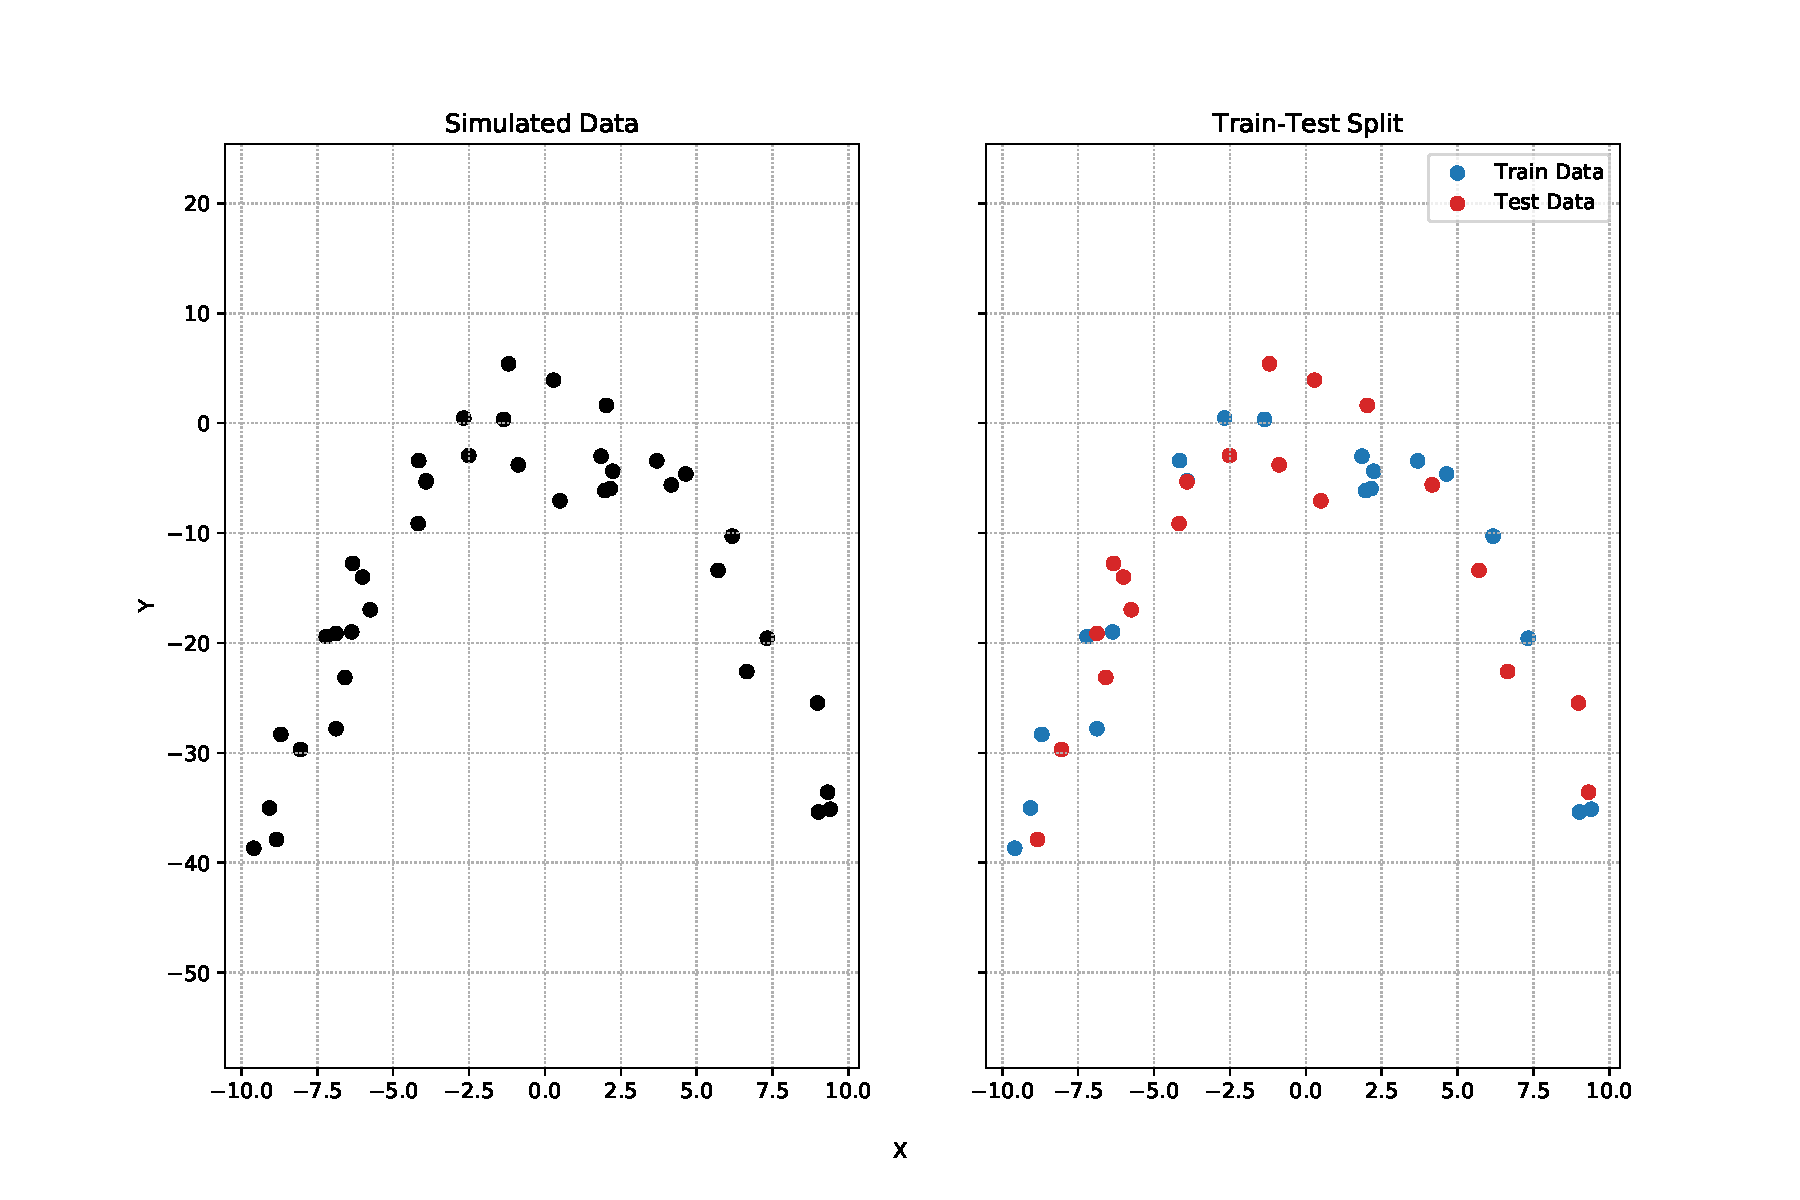
\includegraphics[width=0.5\textwidth]{figures/generated_data_and_splits.pdf}} 
	\subfloat[]{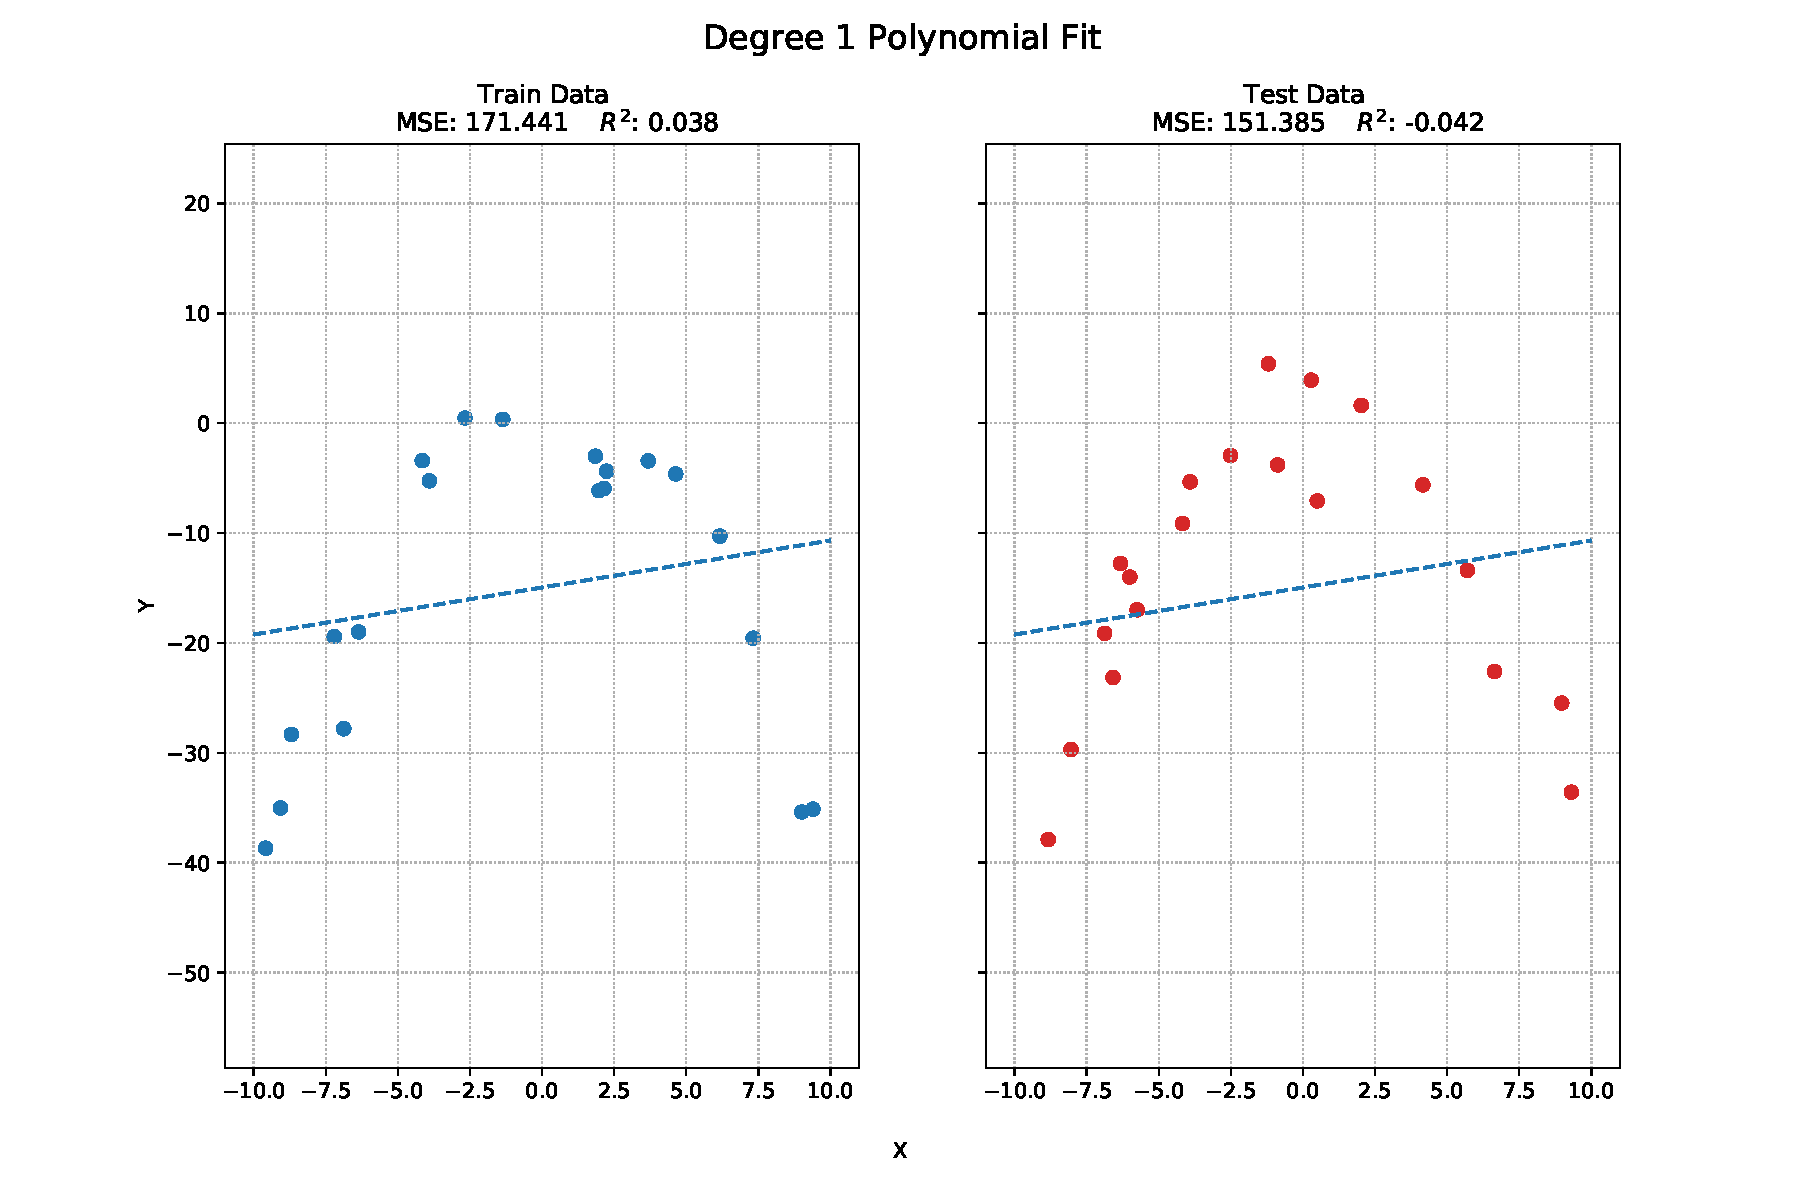
\includegraphics[width=0.5\textwidth]{figures/poly_fit_1.pdf}} \\
	\subfloat[]{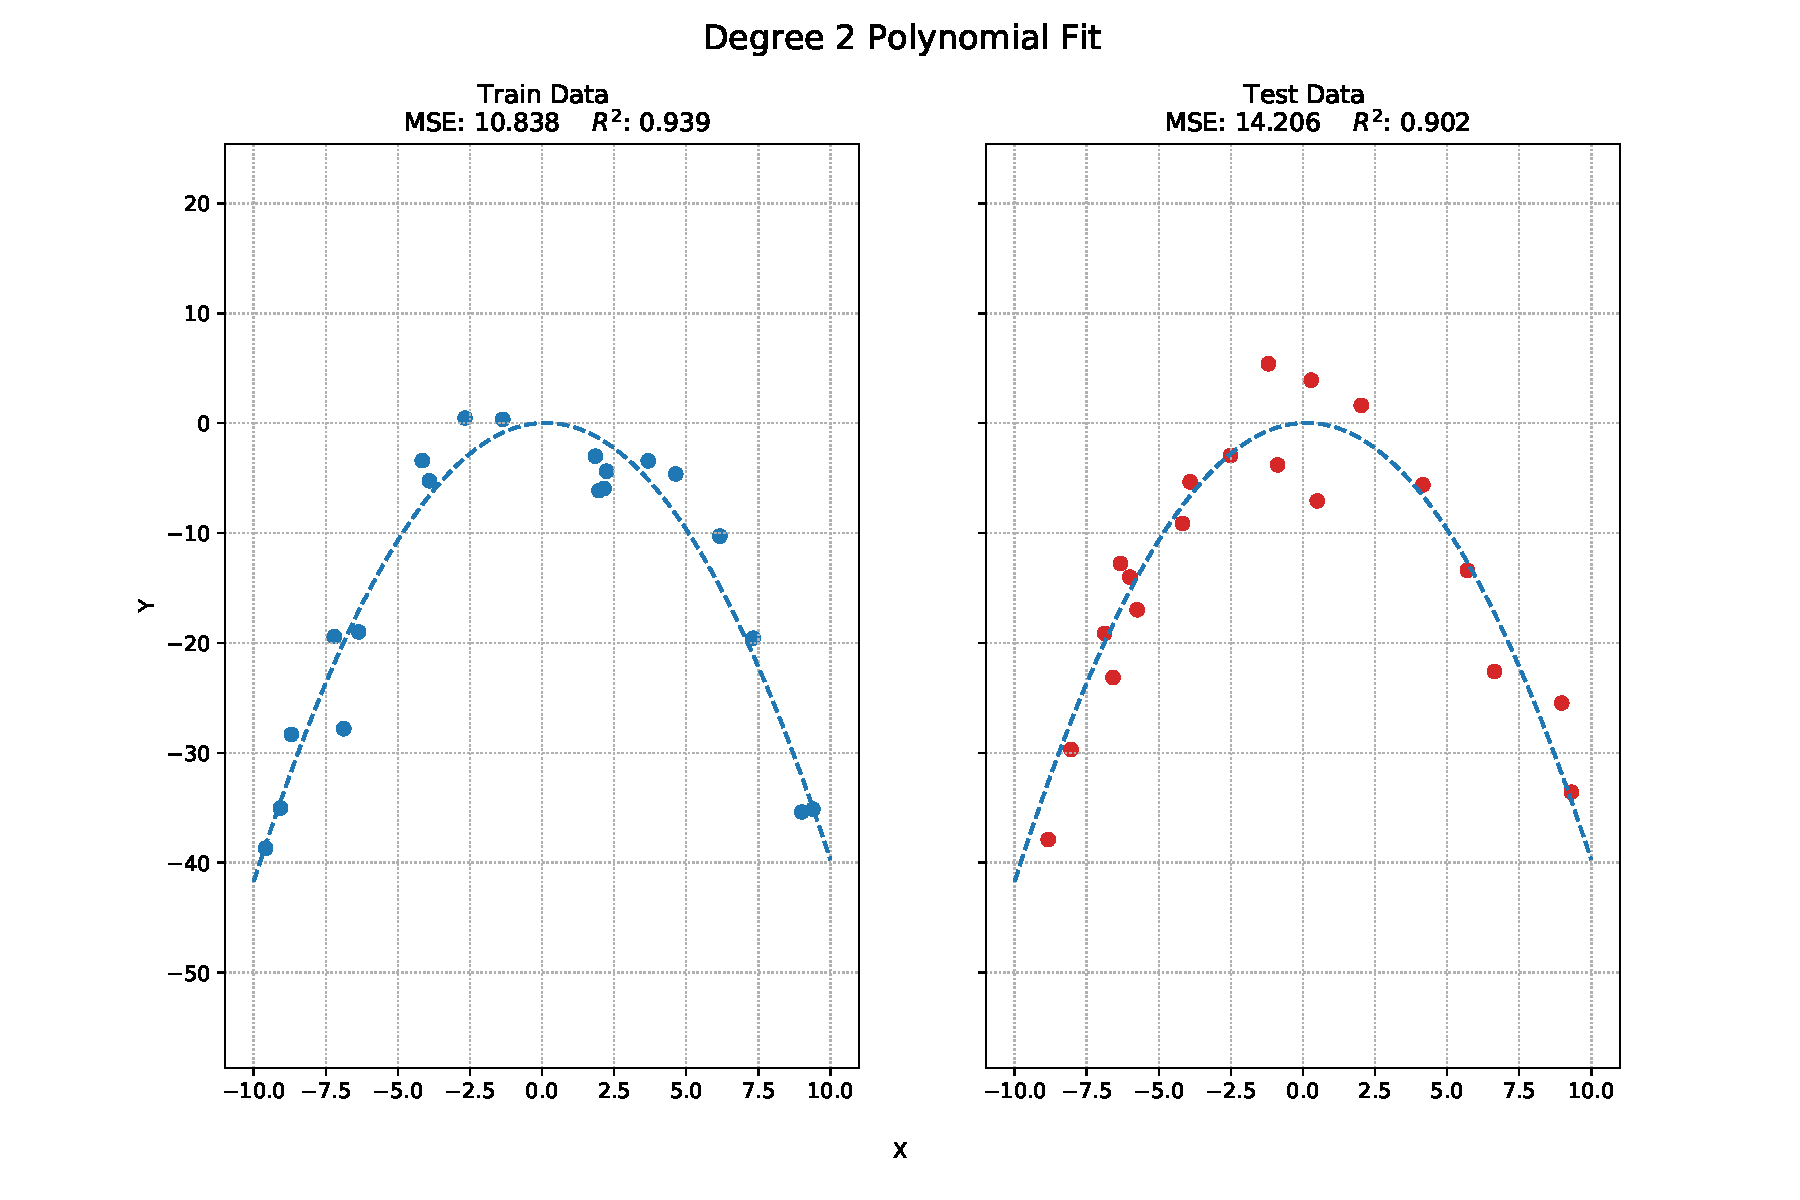
\includegraphics[width=0.5\textwidth]{figures/poly_fit_2.pdf}} 
	\subfloat[]{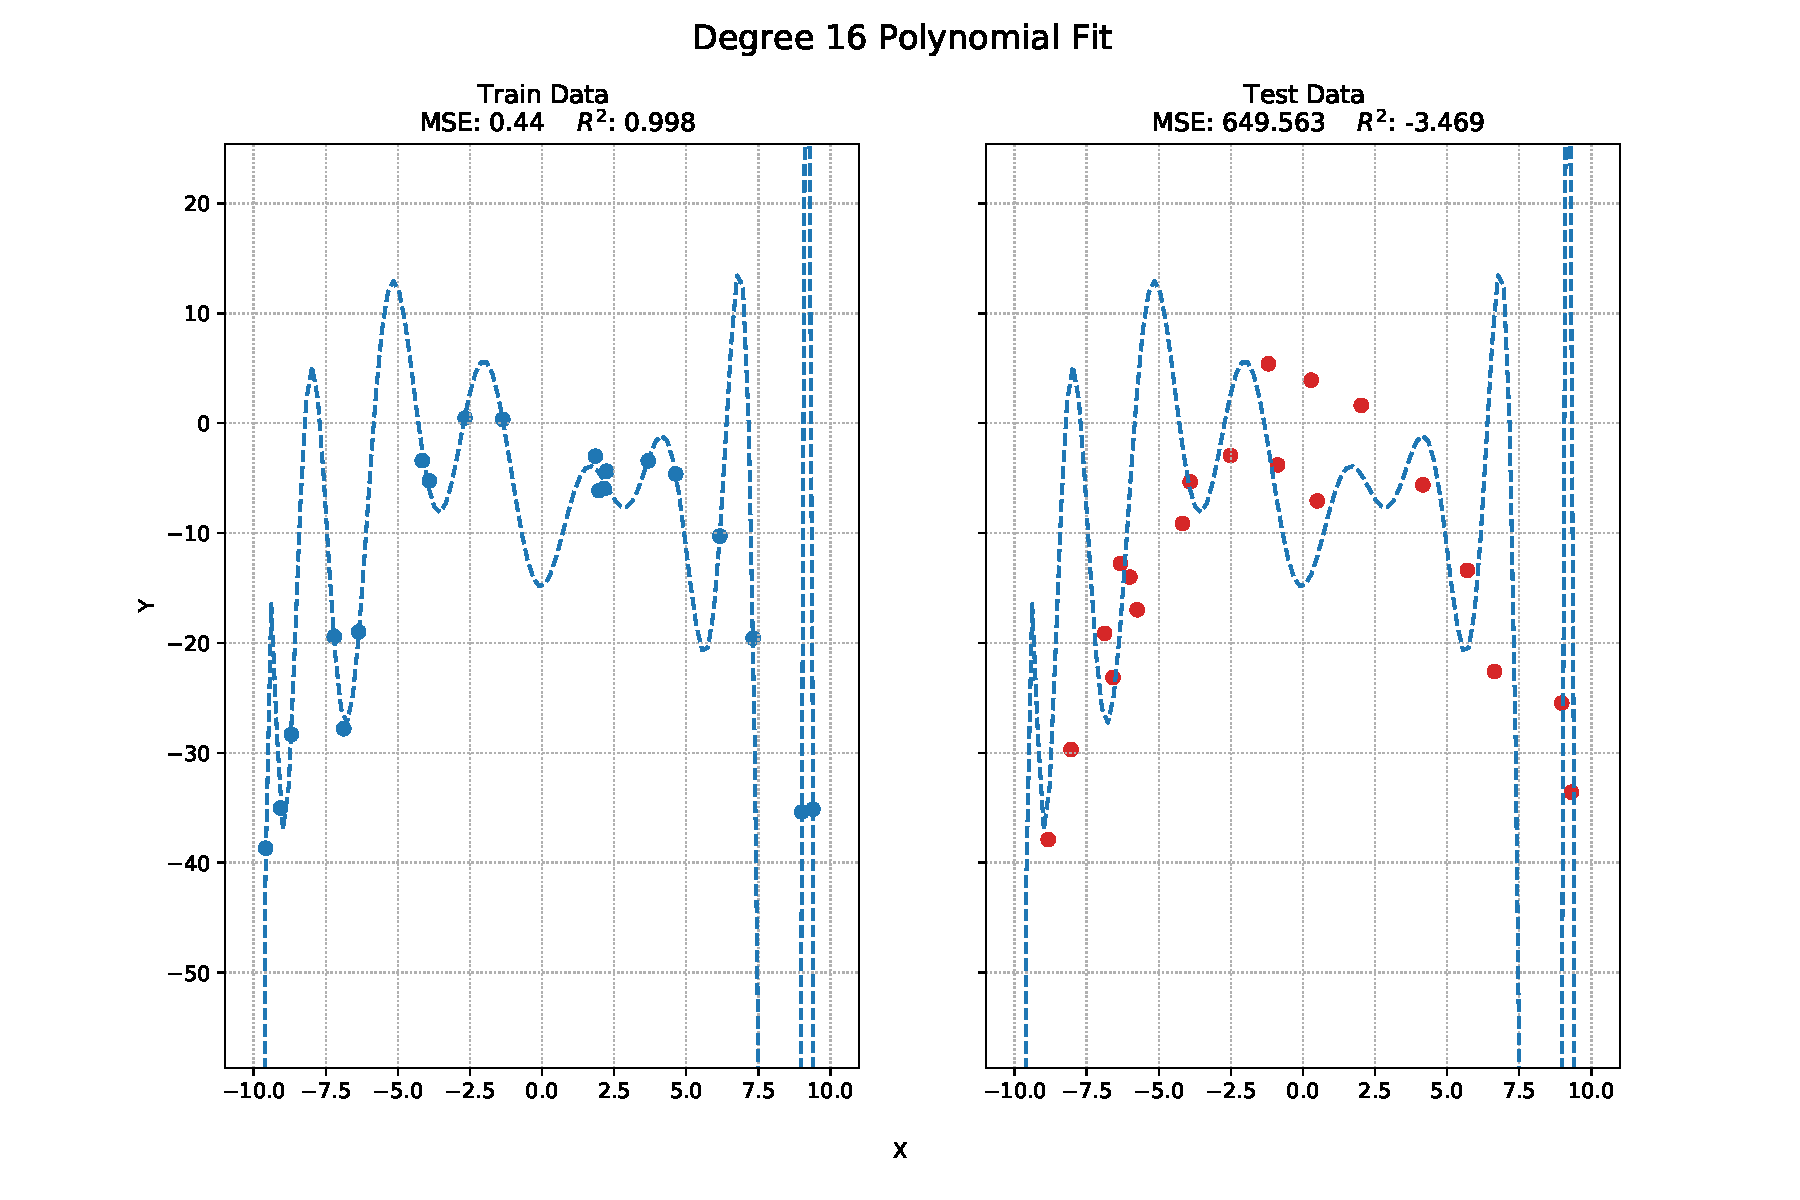
\includegraphics[width=0.5\textwidth]{figures/poly_fit_16.pdf}}
	\caption{Example of how increasing model complexity leads to better model fit on the train-set, but can come at the cost of increasingly worse performance on the test-set. Model fit here is measured visually and in terms of mean-squared-error (MSE) and R squared ($R^2$). The dataset in (a) generated by a degree-2 polynomial with some added noise is split into train and test sets. A degree-1 polynomial underfits the data (b). A more complex degree-2 polynomial improves the fit (c). A far more complex degree-16 polynomial fits the train set extremely well but is overfit as evidenced by its poor test set performance (d).}
	\label{fig:overfitting_example}
\end{figure}

The simplest way to approximate how well a model will perform on unseen data is to "hold-out" a portion of your dataset referred to as a \textit{test-set}, fit your model to the rest of the dataset referred to as the \textit{train-set}, and then check the fit and predictive performance of the model on the test-set. The objective is to create a model that has the best fit and predictive performance on the test-set rather than the train-set. If a model performs noteably worse on the test-set, then you conclude the model is likely overfit and you potentially reject it even though it may be the highest performing model on the train-set. This process is illustrated in Figure \ref{fig:overfitting_example}.  While this method is straightforward and generally effective it does have some drawbacks. The size of the train-set used to train the model is now smaller and may be too small to accurately reflect the model if it were trained on a larger dataset. The selection of which data is divided into the train and test sets may also bias the model and thus bias the estimate of its test-set evaluation. For example, if an essential group or cluster of similar data points are all put into the test-set then the models poor performance on the test-set could be misleading. Cross-validation is an attempt to alleviate these concerns and improve upon this method.

Cross-validation partitions the dataset randomly into K-many sets (with $K \geq 2$). It then uses one of the sets as the test set, and combines the rest into the train-set. The model is fit on the train-set and then evaluated on the test set. This process is then repeated using each of the K sets as the test-set and the average performance across all test-sets becomes the estimate for out of sample performance. In this way the entire dataset is used in both training and testing, helping to alleviate small data or biased train-test splitting concerns.

As you increase the value of K you also increase the size of the train set which gives not only a better model fit but is more likely to overfit if the model itself is prone to overfitting, something we desire to find out. However, increasing the value of K also means you need to train and test the model more times. This is most noticeable when considering the extreme case where K is the size of the dataset, known as leave-one-out cross-validation (LOO-CV). In this case you train the model on all but one data point and then test on the one data point that was left out, and repeat for each data point. While this gives the best estimate of out of sample performance, it requires you to train the model a large number of times. For datasets that number in the thousands or more in the current big data era this can become computationally infeasible. The usual way to deal with this is to reach a compromise by using a smaller value of K, usually 5 or 10. However, applied statisticians have made advancements in the approximation of estimating LOO-CV performance without requiring refitting the model more times than is practical. These methods are rooted in the field of information theory.

- information theory, WAIC and PSIS-LOO
(introduce information theory by briefly mentioning claude shannon?)
- need a better brief introduction to inforation theory, probably cut the below paragraph entirely
The goal of model evaluation is to find the model that will perform best on unseen data, usually measured as its performance on the test-set.
The goal of model fitting and model evaluation is to fit a model on the train-set that maximizes performance relative to some objective, and then hope that this model will continue to perform well on unseen data. While we have described the perils of overfitting and how cross-validation arose as a method to prevent it, this is like defining our objective or criterion which we want to maximize to include regularization. It turns out that there is a branch of mathematics known as Information theory that defines a criterion and a way to maximize it that points to similar goal known as the out-of-sample \textit{deviance}. In information theory, information is formalized into a mathematical formula for information entropy as follows:

\begin{equation}
H(p) = -Elog(p_i) = - \sum_{i=1}^{n} p_i log(p_i)
\end{equation}

In this way, information entropy can be thought of as measuring the uncertainty contained in a probability distribution as the average log-probability of the event (cite Mclreath stat rethink). We can then use this concept of information to reason mathematically about how much one probability distribution differs from another. Specifically, we can compute the average number of extra bits required to represent the data when using our models distribution as compared to the true distribution. This is captured mathematically in the form of Kullback-Leibler divergence (KL divergence) defined as:

\begin{equation}
D_{KL}(p,q) = \sum_{i} p_i (log(p_i) - log(q_i)) = \sum_{i} p_i log \left(\frac{p_i}{q_i} \right)
\end{equation}

The KL divergence can be thought of as the average difference in log probability between the true distribution (\textit{p}) and our models distribution (\textit{q}) (cite mclreath). It gives us a way to compare how similar two distributions are. Note that it does not satisfy some specific mathematical constraints, in particular it is generally not symmetric ($D_{KL}(p,q) \neq D_{KL}(q,p)$), which means KL divergence is not a "measure" or a "distance" in the strict mathematical sense. KL divergence instead represents how much effort is needed to turn one distribution into another, or how much one distribution diverges from another. It is useful because it gives us a rigorous way to compare how similar two distributions are; however, there is one glaring issue of practical significance. The issue is that we do not actually know what the true distribution is (\textit{p}) and therefore we are left with approximating the divergence. It turns out that the true distribution (\textit{p}) is not entirely necessary for comparing models because it is just an additive term which means you can compute the relative difference between models without actually knowing it. Thus, we can use the sum of log probabilities of each observation known as the \textit{log-score}:

\begin{equation}
S(q) = \sum_i log(q_i)
\end{equation}

Relative differences in log-scores will match relative differences in KL divergence. This means that we can compare models via their relative log-score even though the magnitude of the log-score is not easily interpretable. In practice, for Bayesian modelling, we need to average over the posterior distribution (i.e. we need to consider the entire distribution of possible model parameters proportional to how likely they are) and compute a Bayesian log-score known as the \textit{log-pointwise-predictive-density (lppd)}:

\begin{equation} \label{eq:lppd}
lppd(y, \theta) = \sum_i log \frac{1}{S} \sum_s p(y_i | \theta_s)
\end{equation}

The log-score has traditionally been scaled by -2 and referred to as the \textit{deviance}. This is because it has been shown that under general conditions and for many model types a difference between two deviances has a chi-squared distribution (needs a citation). Thus, the factor of 2 would be there to scale the log-score to have this property to make more traditional computations such as likelihood ratio tests more convenient. Modern users now tend to use the lppd itself, especially in a Bayesian context where methods such as likelihood ratio tests are not used.

So it is through Information theory that a way of measuring statistical distance between a models distribution and the target distribution is rigorously defined (KL divergence) and can be approximated in practice (log-score). While the log-score is a principiled way to measure the distance of our model from its target, it has the same flaw that nearly all methods for evaluating models have: the log-score will generally always improve as the model becomes more complex and thus has the potential to overfit the dataset. Researchers have developed a method of evaluation known as \textit{information criteria} which essentially adds a penalty term to the log-score in order to account for increasing model complexity. Thus, as increasingly complex models will generally have a better (lower) log-score, they will need to improve (lower) the log-score by more than the penalty otherwise it is likely they are fitting to random noise and not actually improving general model fit.

The first notable contribution to the development of information criterion was made by (japanese researcher Akaike?). The insight was that for each additional uninformative extra parameter added to a regression model, the test-set deviance becomes worse by a factor about twice the number of parameters. Akaike then showed that this is the case under some general conditions (probably need to cite akaike), and derived what he called \textit{an information criteria} which is now more commonly referred to as Akaike Information Criteria (AIC):

\begin{equation}
AIC = D_{train} + 2k \approx E(D_{test})
\end{equation}

where $D_{train}$ is the deviance on the train-set, $k$ is the number of parameters, and $E(D_{test})$ is the expectation of the deviance on the test-set. Sumio Watanade then generalized AIC to apply to a wider class of models and conditions to develop the Widely Applicable Information Criterion (WAIC), sometimes referred to as Akaike Watanabe Information Criterion:

\begin{equation} \label{eq:waic}
WAIC(y, \theta) = -2 \left( lppd - \sum_i var_{\theta} logp(y_i|\theta) \right)
\end{equation}

where $y$ is the dataset and $\theta$ are the parameters of the model we are evaluating. The $lppd$ is that same as defined in equation \ref{eq:lppd}, and $\sum_i var_{\theta} logp(y_i|\theta)$ is the penalty term which is an estimate of the sum of the variances in the log-likelihood for each observation ($i$) in the dataset. The penalty term is computed by computing the log-likelihood for each sample of parameters from the posterior distribution for the same observation $y_i$ and computing the variance of these log-likelihoods; then repeating this variance computation for each observation $y_i$ in the dataset and summing yields the penalty term. The 2 is there for historical reasons, the same as for computing the deviance in described earlier, and the negative sign before the 2 is to turn the lppd into a postive log-score that we wish to minimize and the penalty term in a positive value that a more complex model needs to "overcome" in order to justify its use.

The WAIC provides a method for estimating the relative KL divergence by estimating the out-of-sample deviance by computing the negative lppd and adding a generalized penalty term that will make the estimate worse (larger) the more complex the model is. WAIC and information criterion in general attempts to estimate the out-of-sample deviance. More recent work attempts to bridge the gap between out-of-sample deviance and cross validation resulting in the current state of the art method for estimating out-of-sample predictive fit that we use for model evaluation in this thesis.

Vethari et al (cite!!!) introduced an efficient computation for estimating LOO-CV from MCMC samples without requiring the repeated re-fitting of the model, referred to as Pareto-Smoothed Importance-Sampling Leave-One-Out cross valdation (PSIS-LOO). Their method also computes the lppd, but instead of adjusting it with the penalty term in \ref{eq:waic}, they use importance sampling to re-weight the log-scores in the lppd to more accurately reflect what the log-scores of each data point would have been if that point had not been used to fit the model, hence the estimation of LOO-CV by re-weighting rather than re-fitting the model. The insight of Vehtari et al. is that the weights needed in order to re-weight the posterior samples for a given datapoint (e.g. the weights $w_s$ for reweighting datapoint $y_1$: $\frac{1}{\sum_s w_s} \sum_s w_s p(y_1 | \theta_s)$) in a manner that resembles what the probability would have been if that datapoint had not actually been observed in the dataset the model was trained on, turns out to be the inverse of the probability that that posterior draw gave to the held out data point (e.g. the weights for $y_1$ are $w_s = \frac{1}{p(y_1|\theta_s)}$). Vehtari et al. further improved the stability of the importance sampling estimates by showing the upper tail of these importance weights fit a generalized Pareto distribution. Instead of using the estimated importance weights themselves, they isntead use the weights to fit a generalized Pareto distribution and then use the weights implied by the fitted Pareto distribution resulting in Pareto smoothed weights. PSIS-LOO is thusly computed as:

\begin{equation} \label{eq:psis-loo}
PSIS-LOO(y, \theta) = \sum_i log \left( \frac{1}{\sum_s w_s^i} \sum_s w_s^i p(y_i | \theta_s) \right)
\end{equation}

where $w_s^i$ is the Pareto-smoothed importance weight for data point $y_i$ with sampled parameters $\theta_s$. The rest is the same as in \ref{eq:lppd} with the key change being the re-weighting performed by multiplying by the weights ($w_s^i$) and re-averaging proportional to the re-weighting ($\sum_s w_s^i$).

The PSIS-LOO estimate is also an estimate of the out-of-sample relative KL divergence. As a result, in practice, the PSIS-LOO estimates are often extremely similar to WAIC estimates. The models that are fit and compared in this thesis all gave near identical results for both PSIS-LOO and WAIC. We have chosen to report just PSIS-LOO in the results section.

\subsubsection{Posterior Predictive Checks}

Posterior predictive checks (PPCs) give us a way to visually check how well a model fits the dataset. Since Bayesian models are generative, we can use the fitted model to simulate values and then observe how closely these generated values resemble the observed dataset. If the distribution of simulated values closely resembles the observed dataset then we say that the model is "well-specified" or is a good fit to the dataset. If the distribution of simulated values does not closely resemble the observed dataset then we say that the model is "misspecified" or is a bad fit to the dataset. It is noteable that PPCs do not only reveal that a model is potentially misspecified but often also give insight into how to potentially improve the model by visually seeing for which data points the model is struggling to fit well. In this way PPCs are not only useful for model evaluation but for model building as well. It was PPCs that lead to the insight of using the Negative Binomial distribution over the Normal and Poisson distributions to fit the sports datasets.

\section{Contribution}

- this should maybe go right after the intro, and then finish with a very short paragraph transitioning to bayesian inference background

The return to play of professional sports during the COVID-19 pandemic presents a unique opportunity to analyze teams playing in situations where home advantage may genuinely no longer apply. The leagues have restricted travel and fan attendance or even created a bubble where only one or two stadiums are used and only the players and necessary staff are present for the games. We consider this restricted return to play as a control group where travel, home stadium familiarity, and home crowd have been controlled (i.e. removed) for enough games to provide a reasonable sample to analyze. There has been considerable academic work analyzing the effect of COVID-19 restrictions on home advantage in European football \cite{Benz2020}. However, comparatively there has been a lack of work analyzing the effect in the North American professional sports leagues. In fact, to the authors knowledge there has only been one work focused on home advantage during COVID-19 across the big four North American professional leagues; and it only investigated the NBA \cite{McHill2020}. In this work, we aim to fill this gap by inferring the effect of and changes in home advantage prior to and during COVID-19 in the big four North American leagues: the National Hockey League (NHL), the National Basketball Association (NBA), Major League Baseball (MLB), and the National Football League (NFL).

We adopt a Bayesian framework to develop a Negative Binomial regression model that adjusts for relative team strengths while inferring home advantage. We choose this approach for two main reasons. First, alternative methods that rely on correlations among raw statistics, such as home win percentage, fail to account for other factors such as relative team strengths. Our regression approach can infer changes in team performance while adjusting for quality of opponents. Second, the Bayesian framework gives more interpretable results and more flexibility in model building than classical regression methods. The Bayesian framework results in distributions for the estimates of each parameter in our model. This allows us to analyze these distributions directly to determine the probability a parameter is greater (less) than a certain value or that it exists in a specific interval, avoiding the confusion that often arises interpreting p-values and confidence intervals.

By examining the resulting home advantage parameter estimates of our model from before and during the COVID-19 pandemic, we can draw conclusions about the existence of the home advantage phenomenon and provide new evidence for its potential causes. We hypothesize that home advantage is a real phenomenon, thus we expect its parameter estimate to drop during the COVID-19 seasons relative to before the COVID-19 seasons. We are also interested in examining if any differences in relative changes in home advantage exist across the leagues as some leagues had different COVID-19 restrictions which could affect home advantage differently. We also show that point totals in North American professional sports are prone to overdispersion, thus, the Negative Binomial distribution allows for better model fit than the more common Poisson and Normal distributions used in regression analyses.
